\documentclass[a4paper,12pt]{article}
\usepackage[T1]{fontenc}
\usepackage[utf8]{inputenc}
\usepackage{lmodern}
\usepackage[french]{babel}
\usepackage{url,csquotes}
\usepackage[hidelinks,hyperfootnotes=false]{hyperref}
%\usepackage[titlepage]{polytechnique}
%\usepackage[titlepage,fancysections,pagenumber]{polytechnique}
\usepackage{float}
\usepackage{graphicx}
\usepackage{subfig}
\usepackage[margin=2cm]{geometry}

\usepackage{tcolorbox}
\usepackage{amsmath}
\usepackage{hyperref}

\usepackage{titlesec}

% Define the font size for subsection headings

%\setcounter{tocdepth}{}
%\usepackage[charter]{mathdesign}

%\setcounter{secnumdepth}{0}


\title{PHY361 DM1 \\
 Oscillations d’atomes piégés dans un potentiel parabolique}
%\subtitle{Stage linguistique à l'IFLS \\
%Formation Préparatoire}
\author{Isai GORDEEV et Imad BARAKAT\\
Promotion X2022, section Escrime}



\begin{document}

\maketitle



\section{Mesure par vol libre de la densité de probabilité de l’impulsion}

\subsection{}

$$E_n = h\omega(n+\frac 1 2) $$

\subsection{}

$a_0 = \displaystyle\sqrt{\frac{\hbar}{2m}} = 72$ nm $ <\ \sim500$ nm, donc nous ne sommes pas capable. 

\subsection{}

image 1(a) est symétrique? spin de Cs? 

Dans l'image a, $p_0 = 0$, après $T_v$ on voit bien que $\psi(p, t)$ s'est séparé.

C'est prévu par la théorie dans le cas libre. Calculons $ |\varphi_1(p)\rangle$ dans la représentation de l'impulsion $p$. 

$$\displaystyle\hat x \overset{P}{=}  i\hbar\frac{\partial}{\partial p} $$
$$\displaystyle\hat p \overset{P}{=} p $$

\begin{equation}
	|\varphi_1(p)\rangle = \hat a^\dagger|\varphi_0(p)\rangle  
\end{equation}

\begin{equation}
	|\varphi_1(p)\rangle =  \left( \frac{\hat x} {a_0}- i\frac{a_0}{\hbar}\hat p \right)|\varphi_0(p)\rangle  
\end{equation}

\begin{equation}
	\varphi_1(p)= \left(i\hbar \frac{1} {a_0}\frac{d}{dp} - i\frac{a_0}{\hbar}p \right)\varphi_0(p) 
\end{equation}

\begin{equation}
	  \varphi_1(p) = \sqrt 2\left(\frac{a_0^2}{\pi \hbar^2}\right)^{\frac14}\left[i\frac{a_op}{\hbar}\exp\left(-\frac{a_0^2}{2\hbar^2}p^2\right)\right] 
\end{equation}

\begin{figure}
	\centering
	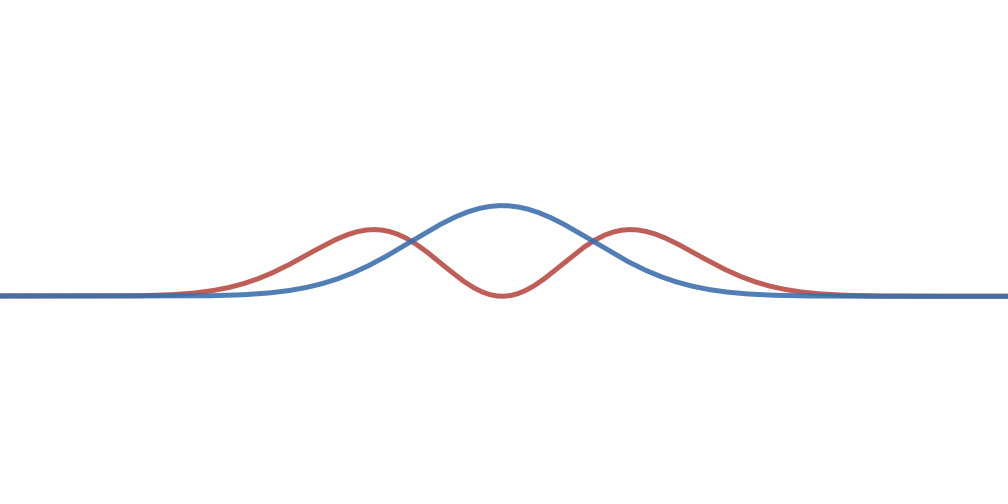
\includegraphics[width=0.7\textwidth]{1}
	\caption{expli}
	\label{fig:image}
\end{figure}

Après l'extinction du laser les atomes de Cs se sont comporté comme les particules libres. 
Enfin, pour calculer $T_v$ il faut mesurer l'impulsion moyenne de $|1\rangle$, ainsi regarder la coordonné de $p_1$. Comme il est demandé de calculer juste l'ordre de grandeur, on va prendre l'ordre de grandeur de $[p_1] = \sqrt 2\frac{\hbar}{a_0}$

\begin{equation}
	T_v = \frac{mx}{[p_1]}  = \frac{mxa_0}{\sqrt 2\hbar}
\end{equation}

\subsection{}
Nous avons déjà utilisé les opérateurs de $\hat x$ et $\hat p$ dans la représentation de l'impulsion $p$ et prouvons maintenant que c'est correct en faisant cet exercice.

\begin{equation}
	|\psi_1\rangle = \hat a^\dagger|\psi_0\rangle  
\end{equation}

\begin{equation}
	|\psi_1\rangle = \left( \frac{a_0}{\hbar}\hat x - \frac{1} {a_0}\hat p\right)|\psi_0\rangle 
\end{equation}


\begin{equation}
		\psi_1(x){=} \left( \frac{a_0}{\hbar}x -i\hbar \frac{1} {a_0}\frac{d}{dx} \right)\psi_0(x) 
\end{equation}


\begin{equation}
	{\displaystyle \psi (x)=\langle x|\psi \rangle =\int \!\!dp~\langle x|p\rangle \langle p|\psi \rangle =\int \!\!\frac{dp}{{\sqrt {2\pi \hbar }}}~{e^{ixp/\hbar }{{\varphi }}(p)},}
\end{equation}

\begin{equation}
	\begin{aligned}
	\displaystyle x\psi (x)&=\langle x|x|\psi \rangle =\int \!\!dp~\langle x|p\rangle \langle p|x|\psi \rangle =\int \!\!\frac{dp}{{\sqrt {2\pi \hbar }}}x{e^{ixp/\hbar }{{\varphi }}(p)} \overset{p.p.}{=} \\ 
	&\int \!\!\frac{dp}{{\sqrt {2\pi \hbar }}}{e^{ixp/\hbar }\underbrace{i\hbar\frac{d}{dp}\varphi(p)}_{\langle p|x|\psi \rangle}} 
\end{aligned}
\end{equation}

\begin{equation}
	\begin{aligned}
		\displaystyle -i\hbar\frac{d}{dx}\psi (x)&=\langle x|p|\psi \rangle =\int \!\!dp~\langle x|p\rangle \langle p|p|\psi \rangle =-i\hbar\frac{d}{dx}\int \!\!\frac{dp}{{\sqrt {2\pi \hbar }}}{e^{ixp/\hbar }{{\varphi }}(p)} {=} \\ 
		&\int \!\!\frac{dp}{{\sqrt {2\pi \hbar }}}{e^{ixp/\hbar }\underbrace{p\varphi(p)}_{\langle p|p|\psi \rangle}} 
	\end{aligned}
\end{equation}

Donc, nous avons dans la p-espace

\begin{equation}\label{eq}
		\varphi_1(p){=} \left( i\hbar\frac1{a_0}\frac{d}{dp} - i \frac{a_0} {\hbar}p \right)\varphi_0(p)(x) 
\end{equation}

\subsection{}

De et de \ref{(eq)}

\begin{equation}\label{key}
	\varepsilon = i\sqrt 2\left(\frac{a^3_0}{\pi\hbar^3}\right)^{\frac14}
\end{equation}

\subsection{}

Regarder dessus 

\section{Préparation du système dans le premier état excité}

\subsection{}











\end{document}